\documentclass[twocolumn,oneside,a4paper,12pt]{article}

% ---------------- Para Modificar ---------------- 
\newcommand{\principal}{Volumes}
\newcommand{\conteudo}{}
\newcommand{\turmas}{3~EMSI~A e do 3~EMSI~B}

\date{abril de 2021}

\newcommand{\citacao}{Que nada nos defina. Que nada nos sujeite. Que a liberdade seja a nossa própria substância.}
\newcommand{\autorcitacao}{Simone de Beauvoir}
% ------------------------------------------------

%-------------------------------------------------
\usepackage[english,brazilian]{babel}
\usepackage[alf]{abntex2cite}
\usepackage[utf8]{inputenc}
\usepackage[T1]{fontenc}
\usepackage[top=15mm, bottom=15mm, left=10mm, right=10mm]{geometry}
\usepackage{framed,booktabs,color,hyperref,graphicx}
\usepackage{amsfonts,amsthm,cancel}
\usepackage{subfigure,enumerate,float}
  
\definecolor{shadecolor}{rgb}{0.8,0.8,0.8}
\pagenumbering{arabic}

% Colunas
\usepackage{multicol}
\columnsep=10mm %Espaçamento entre colunas.
\setlength{\columnseprule}{1pt}

% Cabeçalho
\usepackage{fancyhdr}
\pagestyle{fancy}
\lhead{\textbf{\principal}}
\rhead{}
\renewcommand{\headrulewidth}{1pt} % espessura da linha do cabeçalho
\renewcommand{\footrulewidth}{1pt} % espessura da linha do rodapé

% Parágrafo
\setlength{\parindent}{1.25cm}

\newtheorem{problema}{Problema}
\newtheorem{exercicio}{exercicio}
\newtheorem{exemplo}{Exemplo}
\newtheorem{questao}{Questão}

\usepackage[skip=10pt]{caption}
\captionsetup{font={stretch=0.4,small}}

\newcommand{\FRASE}{\textit{``\citacao ''}\\(\textbf{\autorcitacao})}

\title{\LINHAHORIZONTAL \\\textbf{\\ \principal}\footnote{Resumo para os estudos das aulas não presenciais no período de quarentena para as turmas do \turmas .}\\\LINHAHORIZONTAL}

\newcommand{\LINHAHORIZONTAL}{\center \rule{16cm}{1.25pt}}
\newcommand{\sol}{\textbf{Solução}}

\newcommand{\m}[1]{\(\displaystyle {#1}\)}
\newcommand{\M}[1]{\[{#1}\]}

\author{\textbf{Professor Leandro Vieira}\\EREM Regina Pacis\\Palmeirina-PE}
\newcommand{\frase}{\begin{verse} \flushright{\FRASE} \end{verse}}


\begin{document}
\maketitle

\section{Introdução}

\section{Permutações Caóticas}
O número de permutações caóticas de \(n\) elementos é dado pela fórmula:
\[D_n = n! \cdot \Bigg[\frac{1}{0!} - \frac{1}{1!} + \frac{1}{2!} - \ldots + \frac{(-1)^n}{n!}\Bigg] \]

O número de permutações caóticas de \(n\) elementos é dado por:
\[(n-1)!\]

\begin{exemplo}
Um armário tem três portas, todas com um fechadura com chaves distintas. As chaves foram misturadas, e uma pessoa tem uma única chance de escolher a ordem como recolocá-las nas fechaduras. Qual a probabilidade de que nenhuma das chaves abra a fechadura.
\end{exemplo}

\begin{exemplo}
De quantas formas distintas três argentinos, três brasileiros, dois ingleses e dois franceses podem sentar-se em uma mesa redonda de forma que pessoas de mesma nacionalidade mantenham-se juntas?
\end{exemplo}

\begin{exemplo}
Professores que utilizam quadro branco contam cada vez mais com novas possibilidades de cores a utilizar. Isto facilita principalmente àqueles que lecionam geometria ou mesmo os que desejam colorir pelo simples fato da diversidade. Um professor comprou as 6 canetas abaixo (preta, azul, verde, laranja, vermelha e roxa).

	\begin{figure}[!tbh]
	\center
	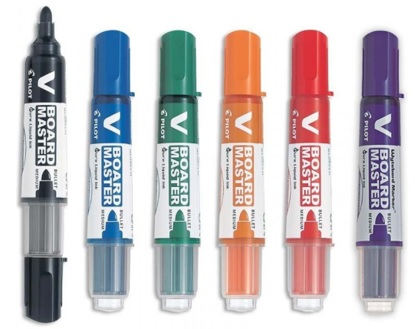
\includegraphics[width=4cm]{p01}
	\end{figure}

\noindent Utilizando todas elas na apresentação de certo conteúdo, ele confundiu-se e errou ao colocar a tampa de todas elas, de forma que nenhuma delas ficou com a tampa correta, correspondente à sua cor. De quantas maneiras distintas essa confusão pode ocorrer?
\end{exemplo}

\begin{exemplo}
Seis cadeiras serão colocadas em torno de uma mesa circular. Nessas cadeiras se sentarão seis pessoas para uma reunião. Sabendo que Carlos e Marcos, são duas das pessoas na reunião, calcule a probabilidade de que eles não se sentem um ao lado outro, uma vez que os locais à mesa serão sorteados.
\end{exemplo}

\begin{exemplo}
Quantas permutações dos inteiros 1, 2, 3, 4, ..., 9, 10 tem exatamente 4 dos números em suas posições originais.
\end{exemplo}

\begin{exemplo}
Com o intuito de separar o lixo para fins de reciclagem, uma instituição colocou em suas dependências cinco lixeiras de diferentes cores, de acordo com o tipo de resíduo a que se destinam: vidro, plástico, metal, papel e lixo orgânico.

	\begin{figure}[!tbh]
	\center
	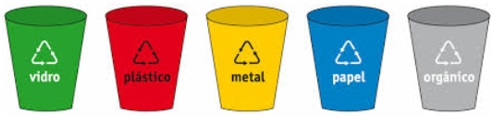
\includegraphics[width=6cm]{p02}
	\end{figure}

\noindent João coleta cinco materiais (um para cada lixeira). Sem olhar para as lixeiras, João joga os cinco resíduos, de modo que todas as lixeiras ficam com apenas um resíduo. Sabendo que apenas dois materiais ficaram nas lixeiras corretas, de quantos modos João pode ter jogado os resíduos?
\end{exemplo}

\begin{exemplo}
Cláudia, Paulo, Rodrigo e Ana brincam entre si de amigo-secreto (ou amigo-oculto). O nome de cada um deles é escrito em pedaços de papel, que são colocados em uma urna, e cada participante retira um desses papéis ao acaso. Qual a probabilidade de que nenhum participante retire seu próprio nome?
\end{exemplo}

\begin{exemplo}
Dois médicos devem examinar, durante uma mesma hora, 6 pacientes, gastando 10 minutos com cada paciente. Cada um dos 6 pacientes deve ser examinado pelos dois médicos.
De quantos modos pode ser feito um horário compatível?
\end{exemplo}

\begin{exemplo}
Uma professora distribui nove livros diferentes para nove crianças. Um mês depois recolhe os livros e, novamente, distribui um livro para cada criança. De quantas maneiras os livros podem ser distribuídos de modo que somente três crianças receba o mesmo livro desta vez?
\end{exemplo}

\begin{exemplo}[\textbf{Extra}]
Em um grupo de colegas de trabalho com 20 pessoas será feito um amigo secreto. Os nomes das 20 pessoas foram colocadas em uma urna, e cada um vai tirar um nome correspondente. Qual a probabilidade que ninguém tire seu próprio nome:
\end{exemplo} 

\end{document}